\documentclass[a4paper, 11pt]{article}
\usepackage[cpp]{mypackage}
\usepackage{float}
\usepackage{amsmath}
\usepackage{graphicx}
\usepackage{geometry}
\geometry{scale=0.8}
% \linespread{1.5}
\usepackage[colorlinks,linkcolor=red]{hyperref}

\title{
\normalfont \normalsize
\textsc{School of Data and Computer Science, Sun Yat-sen University} \\ [25pt] %textsc small capital letters
\rule{\textwidth}{0.5pt} \\[0.4cm] % Thin top horizontal rule
\huge  Lab3 Othello Game ($\alpha-\beta$ pruning) \\ % The assignment title
\rule{\textwidth}{2pt} \\[0.5cm] % Thick bottom horizontal rule
\author{17341015 Hongzheng Chen}
\date{\normalsize\today}
}

\begin{document}
\maketitle
\tableofcontents
\newpage

\section{Othello}
Othello (or Reversi) is a strategy board game for two players, played on an $8 \times 8$ uncheckered board. There are sixty-four identical game pieces called disks (often spelled "discs"), which are light on one side and dark on the other. Please see figure \ref{fig:othello}.

Players take turns placing disks on the board with their assigned color facing up. During a play, any disks of the opponent's color that are in a straight line and bounded by the disk just placed and another disk of the current player's color are turned over to the current player's color.

The object of the game is to have the majority of disks turned to display your color when the last playable empty square is filled.
\begin{figure}
  \centering
  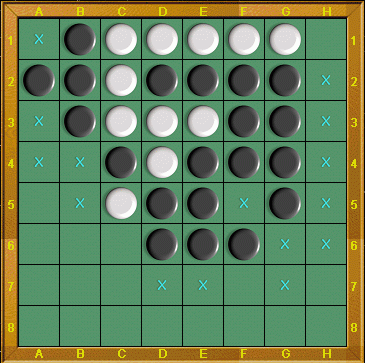
\includegraphics[width=6cm]{fig/othello}
  \qquad
  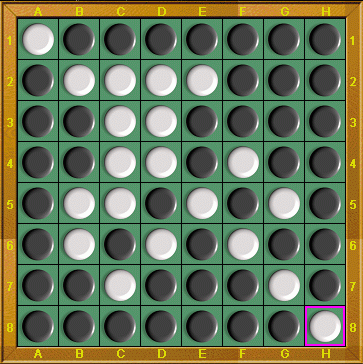
\includegraphics[width=6cm]{fig/othello2}
  \caption{Othello Game}
  \label{fig:othello}
\end{figure}

You can refer to \url{http://www.tothello.com/html/guideline_of_reversed_othello.html} for more information of guideline, meanwhile, you can download the software to have a try from \url{http://www.tothello.com/html/download.html}. The game installer \texttt{tothello\_trial\_setup.exe} can also be found in the current folder.


\section{Tasks}
\begin{enumerate}

\item In order to reduce the complexity of the game, we think the board is $6\times 6$.

\item There are several evaluation functions that involve many aspects, you can turn to \url{http://blog.sina.com.cn/s/blog_53ebdba00100cpy2.html} for help. In order to reduce the difficulty of the task, I have given you some hints of evaluation function in the file \texttt{Heuristic Function for Reversi (Othello).cpp}.

\item Please choose an appropriate evaluation function and use min-max and $\alpha-\beta$ prunning to implement the Othello game. The framework file you can refer to is \texttt{Othello.cpp}. Of course, I wish your program can beat the computer.

\item Write the related codes and take a screenshot of the running results in the file named \textsf{E03\_YourNumber.pdf}, and send it to \textsf{ai\_201901@foxmail.com}.
\end{enumerate}


\section{Codes}
The codes below only show the search part and the judge part.
For other parts, please refer to the attached \verb'Othello.cpp'.

Since this \LaTeX template cannot insert Chinese, so I only screenshot the minimax search algorithm here.
\begin{figure}[H]
  \centering
  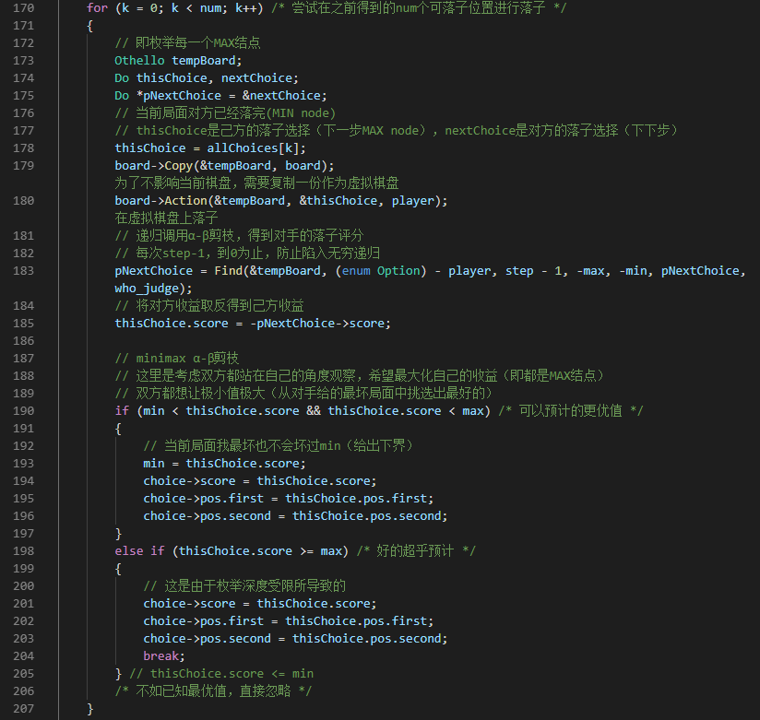
\includegraphics[width=\linewidth]{fig/code.png}
\end{figure}

I modify the provided heuristics to $6\times 6$ game, and the code is shown below.
There is lots of aprior knowledge and filled with magic numbers!
\begin{lstlisting}
  double Othello::MyJudge(Othello *board, enum Option player)
  {
    int my_tiles = 0, opp_tiles = 0, i, j, k, my_front_tiles = 0, opp_front_tiles = 0, x, y;
    double p = 0, c = 0, l = 0, m = 0, f = 0, d = 0;
    enum Option my_color = player;
    enum Option opp_color = (enum Option) - player;

    // eight directions
    int X1[] = {-1, -1, 0, 1, 1, 1, 0, -1};
    int Y1[] = {0, 1, 1, 1, 0, -1, -1, -1};
    // aprior weights for each movement
    int V[6][6] =
      {{20, -3, 11, 11, -3, 20},
       {-3, -7, -4, -4, -7, -3},
       {11, -4, 2, 2, -4, 11},
       {11, -4, 2, 2, -4, 11},
       {-3, -7, -4, -4, -7, -3},
       {20, -3, 11, 11, -3, 20}};

    // Piece difference
    for (i = 0; i < 6; i++)
      for (j = 0; j < 6; j++)
      {
        // count how many tiles are occupied
        if (board->cell[i][j].color == my_color)
        {
          d += V[i][j];
          my_tiles++;
        }
        else if (board->cell[i][j].color == opp_color)
        {
          d -= V[i][j];
          opp_tiles++;
        }

        // find the difference in eight directions
        if (board->cell[i][j].color != SPACE)
        {
          for (k = 0; k < 8; k++)
          {
            x = i + X1[k];
            y = j + Y1[k];
            if (x >= 0 && x < 6 && y >= 0 && y < 6 && board->cell[x][y].color == SPACE)
            {
              if (board->cell[i][j].color == my_color)
                my_front_tiles++;
              else
                opp_front_tiles++;
              break;
            }
          }
        }
      }

    // calculate the proportions
    if (my_tiles > opp_tiles)
      p = (100.0 * my_tiles) / (my_tiles + opp_tiles);
    else if (my_tiles < opp_tiles)
      p = -(100.0 * opp_tiles) / (my_tiles + opp_tiles);
    else
      p = 0;

    if (my_front_tiles > opp_front_tiles)
      f = -(100.0 * my_front_tiles) / (my_front_tiles + opp_front_tiles);
    else if (my_front_tiles < opp_front_tiles)
      f = (100.0 * opp_front_tiles) / (my_front_tiles + opp_front_tiles);
    else
      f = 0;

    // Corner occupancy
    my_tiles = opp_tiles = 0;
    if (board->cell[0][0].color == my_color)
      my_tiles++;
    else if (board->cell[0][0].color == opp_color)
      opp_tiles++;
    if (board->cell[0][5].color == my_color)
      my_tiles++;
    else if (board->cell[0][5].color == opp_color)
      opp_tiles++;
    if (board->cell[5][0].color == my_color)
      my_tiles++;
    else if (board->cell[5][0].color == opp_color)
      opp_tiles++;
    if (board->cell[5][5].color == my_color)
      my_tiles++;
    else if (board->cell[5][5].color == opp_color)
      opp_tiles++;
    c = 25 * (my_tiles - opp_tiles);

    // Mobility
    // The more tiles can be moved on, the better
    my_tiles = Rule(board, my_color);
    opp_tiles = Rule(board, opp_color);
    if (my_tiles > opp_tiles)
      m = (100.0 * my_tiles) / (my_tiles + opp_tiles);
    else if (my_tiles < opp_tiles)
      m = -(100.0 * opp_tiles) / (my_tiles + opp_tiles);
    else
      m = 0;

    // final weighted score (magic numbers!)
    double score = (10 * p) + (801.724 * c) +  (78.922 * m) + (74.396 * f) + (10 * d);
    return score;
  }
\end{lstlisting}

\section{Results}
I let the two AIs play with each other, and the results are shown below.
\begin{figure}[H]
  \centering
  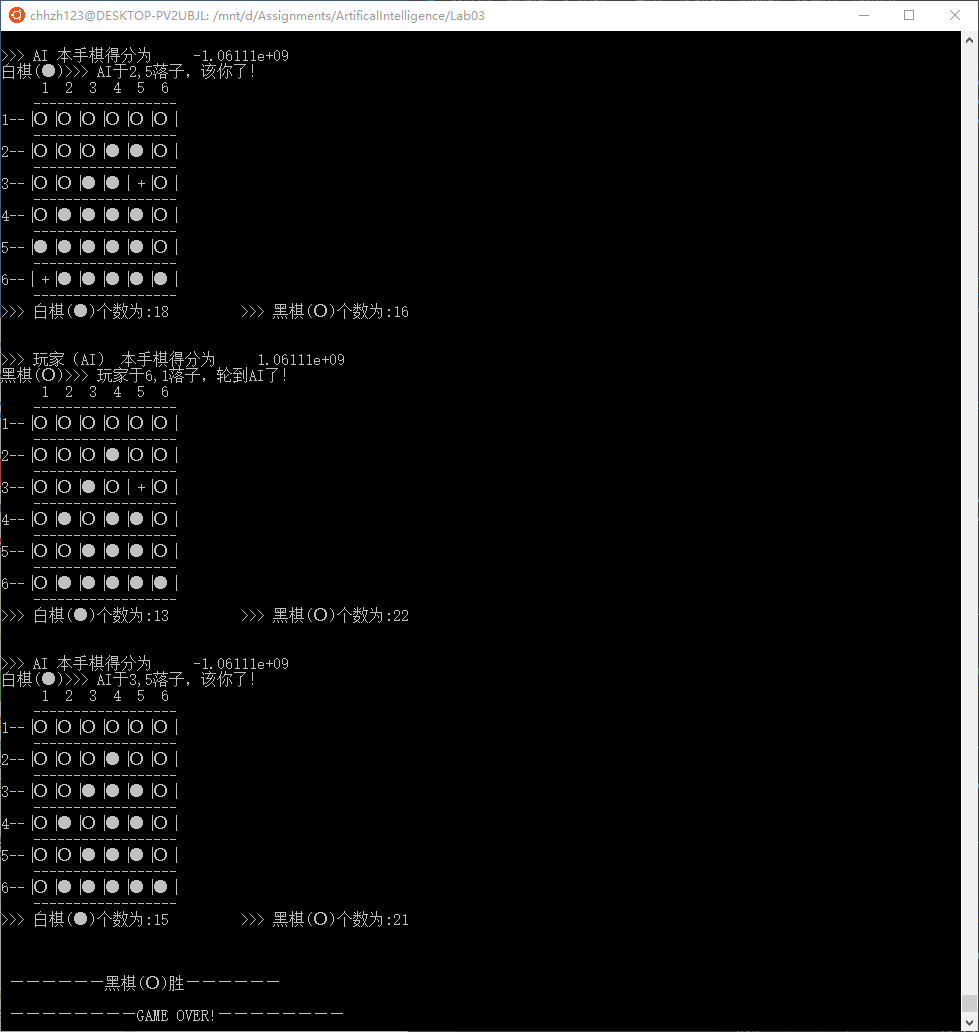
\includegraphics[width=\linewidth]{fig/black.png}
  \caption{My AI uses \textbf{black} disk and beats the computer}
\end{figure}
\begin{figure}[H]
  \centering
  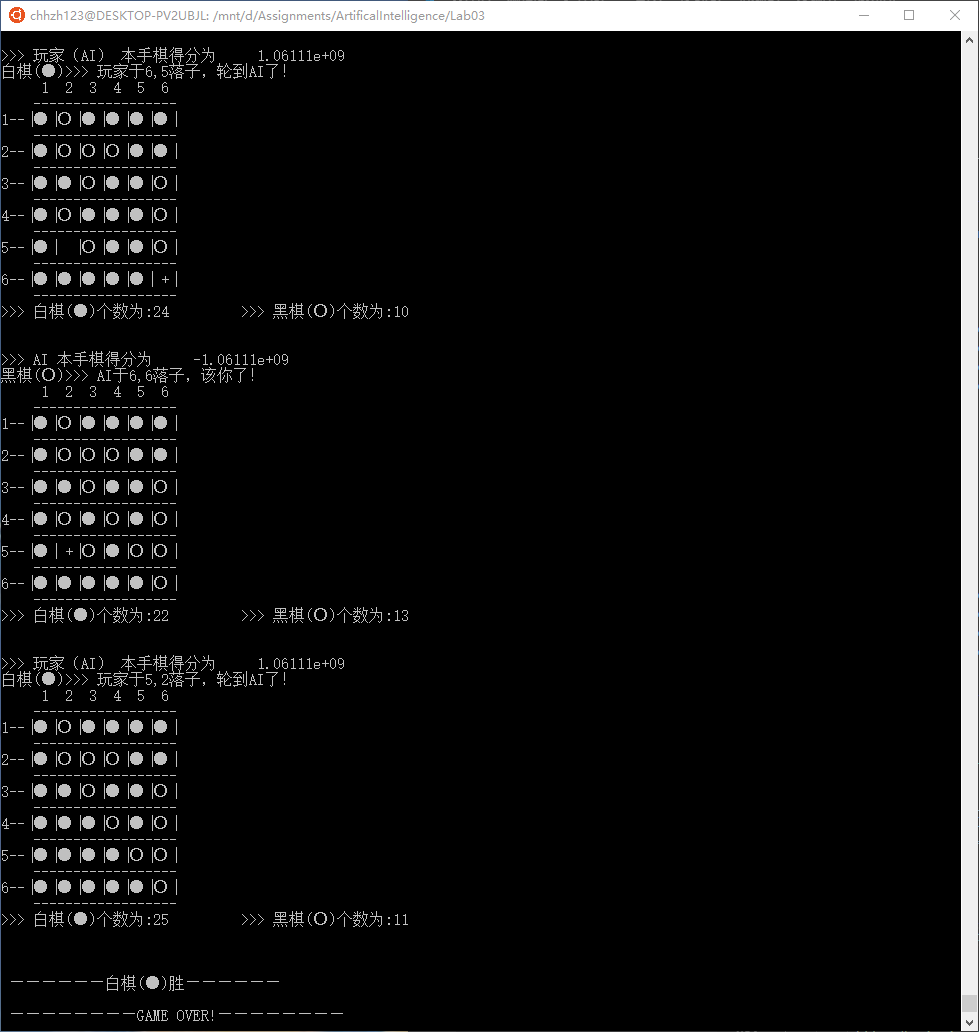
\includegraphics[width=\linewidth]{fig/white.png}
  \caption{My AI uses \textbf{white} disk and beats the computer}
\end{figure}

% http://othelloacademy.blogspot.com/p/strategies.html

\end{document}